\documentclass[a4paper]{article}
\usepackage[warn]{mathtext}
\usepackage[utf8]{inputenc}
\usepackage[T2A]{fontenc}
\usepackage[english,russian]{babel}
\usepackage{indentfirst}
\usepackage{misccorr}
\usepackage{subcaption}
\captionsetup{compatibility=false}
\usepackage{geometry}
\geometry{verbose,a4paper,tmargin=2cm,bmargin=2cm,lmargin=1.5cm,rmargin=1.5cm}
\usepackage{graphicx}
\usepackage{wrapfig}
\usepackage{amsmath}
\usepackage{fancyhdr}
\usepackage{floatflt}
\usepackage{float}
\usepackage{amssymb}
\usepackage{color}
\usepackage{lscape}
\usepackage{hvfloat}
\usepackage{amsfonts}
\usepackage{euscript}
\usepackage{newunicodechar}
\usepackage{booktabs}
\usepackage{multirow}

\begin{document}

\graphicspath{ {pictures/} }

\begin{titlepage}
	\centering
	\vspace{5cm}
    {\scshape\LARGE Московский физико-технический институт\par}
	\vspace{5cm}
	{\scshape\Large Лабораторная работа по общей физике \par}
	\vspace{1cm}
    {\huge\bfseries  5.1 Измерение коэффициента ослабления $\gamma$-лучей в веществе
    и определение их энергий \par}
	\vspace{1cm}
	\vfill
    \begin{flushright}
        {\large выполнила студент Б01-907 группы}\par
        \vspace{0.3cm}
        {\LARGE Юлия Прохорова}
    \end{flushright}
	\vfill
Долгопрудный, 2021
% Bottom of the page
\end{titlepage}

\pagestyle{fancy} 
\fancyhead[L]{5.1}
\fancyhead[R]{Юлия Прохорова}
\fancyhead[C]{}
\fancyfoot[C]{ \noindent\rule{\textwidth}{0.4pt} \thepage }

\tableofcontents

\newpage



\section{Цель работы}

\begin{enumerate}
    \item  C помощью сцинтилляционного счетсчика измерить линейные кожффициенты ослабления потока $\gamma$ - лучей в свинце,
    железе и алюмини
    \item  По их величине определить энергию $\gamma$ - квантов
\end{enumerate}



\section{Теория}

Гамма-лучи возникают при переходе возбужденных ядер из одного состояние в другое, более низкое. 
$E_{\gamma}$ лежит в значениях от 10 кэВ до 1000 кэВ. При проходе через вещество, пучок ослабляется по закону:

\begin{equation}
    I = I_0 e^{-\mu l}
\end{equation}

\begin{equation}
    I = I_0 e^{-\mu' m_1}
\end{equation}

$I, \; I_0$ - интенсивности прошедшего и падающего излучений, $l$  - длина пути, $m_1$ - масса 
пройденного вещества на единицу площади, $\mu$ и $\mu'$ - константы, зависящие от вещества. $\mu'$ 
не зависит от плотности вещества. \par 

Ослабление потока $\gamma$ - лучей связано стремя эффетками: 
\begin{enumerate}
    \item фотоэлектрическое поглощение
    \item комптоновское рассеяние
    \item генерация электрон-позитронных пар
\end{enumerate}



\subsection{Фотоэлектрическое поглощение}

При столкновении $\gamma$ - квантов с электронами внутренних атомных оболосчек может происходить поглощение 
квантов. Энергия кванта передается электрону, а импульс делится между электроном и ионом. Наружные электроны 
не принимают участия в фотоэлектрическом поглощении, т.к. они почти свободные и слабо связаны с ядром. \par 

Вероятность $dP_ф$ фотоэлектрического поглощения гамма-квантов пропорциональна длине пути $dl$ и плотности 
электронов в среде:

\begin{equation}
    dP_ф = \sigma_ф n_1 dl
\end{equation}

$n_1$ - плотность внутренних электронов, $\sigma_ф$ - поперечное сечение фотожлектрического поглощения, 
оно характеризует вероятность фотоэффекта, рассчитанную на один электрон. \par 

Найдем связь между коэффициентом поглощения для фотоэффекта $\mu_ф$ и сечением $\sigma_ф$:

\begin{equation}
    \mu_ф = \sigma_ф n_1
\end{equation}

Эта формула отражает зависимость $\mu_ф$ от плотности среды в явном виде.\par 

Пусть в результате фотоэффетка энергия $\gamma$-кванта передается электрону на $i$ оболочке, 
$W_i$ - энергия связи этого электрона. Тогда кинетическая энергия электрона:

\begin{equation}
    T_i = \hbar \omega - W_i
\end{equation}

на вакантное место могут перейти электроны с соседних оболчек, при таких переходах возникает характеристическое 
рентгеновское излучение, которое, например, в РЭМ используется в режиме рентгеновской спеткроскопии для определения 
состава образца. \par 

Вероятность фотоэффекта сложно зависит от энергии гамма-лучей и от заряда ядер:

\begin{equation}
    \sigma_ф \propto \frac{Z^5}{(\hbar \omega)^{2,5}}
\end{equation}

Эта формула отражает такую зависимость (рис. \ref{p1})

\begin{figure}[H]
    \begin{center}
    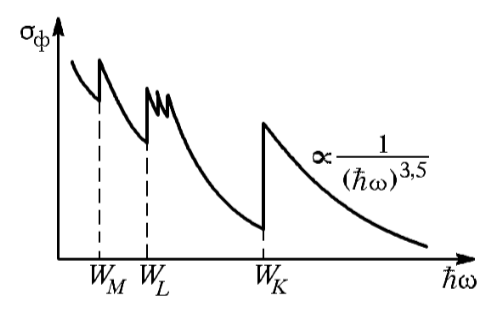
\includegraphics[scale = 0.8]{p1.png}
    \caption{Зависимость сечения фотоэффекта от энергии $\gamma$-квантов}
    \label{p1}
    \end{center}
\end{figure}

Вероятность фотоэффекта быстро возрастает при переходе от легких к тяжелым элементам и резко падает
с увеличением энергии гамма-квантов. При возрастании энергии сечение скачкообразно возрастает, когда 
становится возможным выбивание электронов с очередной оболочки. Фотоэффект является доминирующим механизмом
поглощения гамма-квантов при не очень высоких энергиях.



\subsection{Комптоновское рассеяние}

Комптон эффект - упругое столкговение гамма-кванта с электроном. Этот эффект происходит на свободных 
или слабосвязанных электронах в отличие от фотоэффекта. Роль эффекта Комптона становиться существенной 
только когда энергия гамма-квантов становится много больше энергии связи электронов в атоме. Атомные электроны
можно считать практиески свободными. \par 

Вертоятность Комптон эффекта сложно зависит от энергии гамма-квантов. В случае, когда энергия 
гамма-кванта много больше энергии покоя электрона:

\begin{equation}
    \sigma_k = \pi r^2 \frac{mc^2}{\hbar \omega} \left ( \ln{\frac{2 \hbar \omega}{mc^2}}+ \frac{1}{2} \right )
\end{equation}

$r \approx 2.8 \cdot 10^{-13} \; см$ - классический радиус электрона. Следует, что сечение комптон-эффекта 
с ростом энергии фотонов падает не так резко, как сечение фотоэффекта. \par 

Сечение $\sigma_k$ относится к одному свободному электрону, а сечение фотоэффекта рассчитано на атом. 
Значит комптоновское рассеяние становится в $Z$ раз больше. \par 

Комптоновский коэффициент линейного ослабления $\mu_k$ связан с сечением $\sigma_k$ через плотность слабосвязанных 
электронов $n$:

\begin{equation}
    \mu_k = \sigma_k \cdot n
\end{equation}

Отметим, что эффект Комптона приводит не к поглащению, а к рассеянию гамма-кватнов. 



\subsection{Генерация электрон-позитронных пар}

При энергиях $\gamma$-лучей, превышающих $2mc^2 = 1.02 \; МэВ$, становится возможен процесс образования 
электрон-позитронных пар. Рождение пар происходит в эл. поле ядер, вероятность процесса $\sim \; Z^2$ и сложным
образом зависит от энергии фотона. \par 

При энергиях более 1.02 МэВ фотоэффект почти не играет роли даже для самых тяжелых ядер. Вероятность образования пар 
сравнительна с вероятностью комптоновского рассеяние. Рождение пар существенно только для самых тяжелых элементов. 
Для свинца вероятность рождения пар сравнивается с вероятностью комптоновского эффекта только при 4.7 МэВ.



\subsection{Полный коэффициент ослабления}

Полный линейный кожффициент $\mu$ равен сумме коэффициентов для всех трех рассмотренных процессов.
На рис. \ref{p2}

\begin{figure}[H]
    \begin{center}
    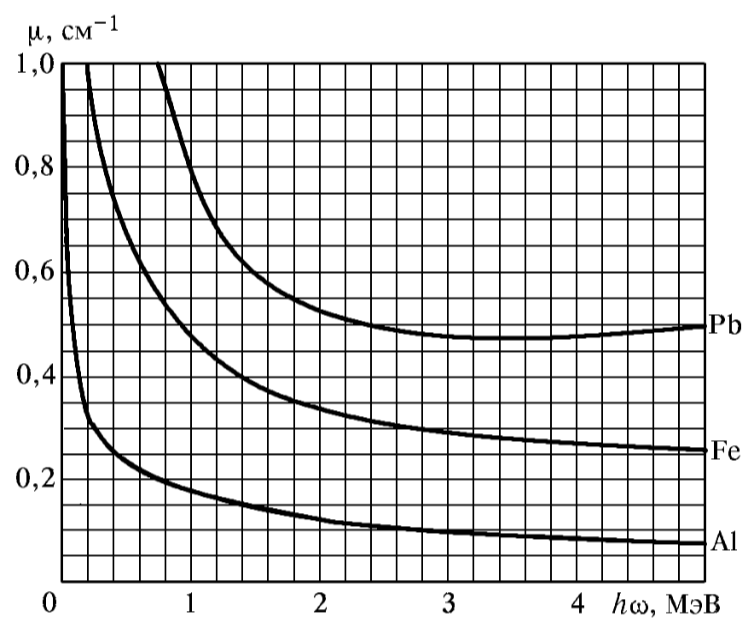
\includegraphics[scale = 0.8]{p2.png}
    \caption{Полные коэффициенты ослабления потока $\gamma$ - лучей в алюминии, железе и свинце}
    \label{p2}
    \end{center}
\end{figure}

% Please add the following required packages to your document preamble:
% \usepackage{multirow}
\begin{table}[H]
    \begin{center}
    \begin{tabular}{|l|l|l|l|}
    \hline
    \multicolumn{1}{|c|}{\multirow{2}{*}{МэВ}} & \multicolumn{3}{c|}{Коэффициент   поглощения, 1/c} \\ \cline{2-4} 
    \multicolumn{1}{|c|}{}                     & Al              & Fe             & Pb              \\ \hline
    0,1                                        & 0,459           & 2,930          & 63,000          \\ \hline
    0,2                                        & 0,329           & 1,150          & 11,300          \\ \hline
    0,3                                        & 0,281           & 0,866          & 4,570           \\ \hline
    0,4                                        & 0,250           & 0,740          & 2,630           \\ \hline
    0,5                                        & 0,288           & 0,662          & 1,830           \\ \hline
    0,6                                        & 0,210           & 0,606          & 1,420           \\ \hline
    0,7                                        & 0,196           & 0,563          & 1,170           \\ \hline
    0,8                                        & 0,184           & 0,528          & 1,010           \\ \hline
    0,9                                        & 0,175           & 0,498          & 0,891           \\ \hline
    1,0                                        & 0,166           & 0,472          & 0,806           \\ \hline
    1,1                                        & 0,158           & 0,450          & 0,740           \\ \hline
    1,2                                        & 0,151           & 0,430          & 0,688           \\ \hline
    1,3                                        & 0,145           & 0,413          & 0,648           \\ \hline
    1,4                                        & 0,140           & 0,398          & 0,617           \\ \hline
    1,5                                        & 0,135           & 0,384          & 0,592           \\ \hline
    1,6                                        & 0,131           & 0,372          & 0,573           \\ \hline
    1,7                                        & 0,127           & 0,362          & 0,556           \\ \hline
    1,8                                        & 0,123           & 0,352          & 0,543           \\ \hline
    1,9                                        & 0,120           & 0,343          & 0,532           \\ \hline
    2,0                                        & 0,117           & 0,335          & 0,523           \\ \hline
    2,1                                        & 0,114           & 0,328          & 0,515           \\ \hline
    2,2                                        & 0,111           & 0,322          & 0,508           \\ \hline
    2,3                                        & 0,109           & 0,316          & 0,503           \\ \hline
    2,4                                        & 0,107           & 0,310          & 0,498           \\ \hline
    2,5                                        & 0,104           & 0,306          & 0,494           \\ \hline
    2,6                                        & 0,103           & 0,301          & 0,490           \\ \hline
    2,7                                        & 0,101           & 0,296          & 0,487           \\ \hline
    2,8                                        & 0,099           & 0,292          & 0,485           \\ \hline
    2,9                                        & 0,097           & 0,289          & 0,482           \\ \hline
    3,0                                        & 0,096           & 0,285          & 0,480           \\ \hline
    \end{tabular}
    \caption{Коэффициент поглощения разных веществ}
    \end{center}
    \end{table}

Получим формулу (1). Рассмотрим опыты в хорошей геометрии, когда $\gamma$ - кванты выводит из пучка фотоэлектрическое поглощение, комптоновское
рассеяние и генерация пар. \par 

При прохождении через вещество меняется количество, а не энергия квантов в пучке, значит коэффициент 
$\mu$ не зависит от длины пути. Пусть $-dN$ число гамма-квантов, выбывших из пучка на пути $dl$, это число 
пропорционально имеющемуся их числу $N$ и пройденному пути $dl$:

\begin{equation}
    -dN = \mu N dl
\end{equation}

Интегрируем от нулевой толщины до заданной:

\begin{equation}
    N = N_0 e^{-\mu l}
\end{equation}

Получили ф-лу (1).\par 

В плохой геометрии, когда рассеянные под небольшими углами кванты остаются в пучке эта формула не применима, однако,
хорошо работает :). \par
Причина хорошего согласия в том, что гамма-кванты с энергие 1-2 МэВ, потерявшие энергию из-за комптоновского ослабления, 
быстро выбывают из пучка аз-за резкого увеличения сечений $\sigma_ф$ и $\sigma_k$. В данной работе коэффициент ослабления $\mu$
измеряектся в хорошей геометрии:

\begin{equation}
    \mu = \frac{1}{l} \ln{\frac{N_0}{N}}
\end{equation}



\section{Экспериметнальная установка}

Схема установки показана на рис. \ref{setup1}
Свинцовый коллиматор выделяет узкий параллельный пучок гамма-квантов, проходящий через набор поглотителей П.
Сигналы от счетсчика усиливаются и регистрируются пересчетным приьором ПП. \par 

При недостаточно хорошей геометрии в результате опытов могут быть погрешности. В реальности всегда имеется 
вероятность, что гамма-квант провзаимодействует в поглатителе несколько раз до того, как попадет в детектор (рис. \ref{setup2})
Чтобы этого избежать сцинтилляционный счетсчик расположен на больом расстоянии от источника гамма-квантов, а полглотители 
имеют небольшие размеры, также поглотители следует размещать на небольшом расстоянии друг от друга. 

\begin{figure}[H]
    \begin{center}
    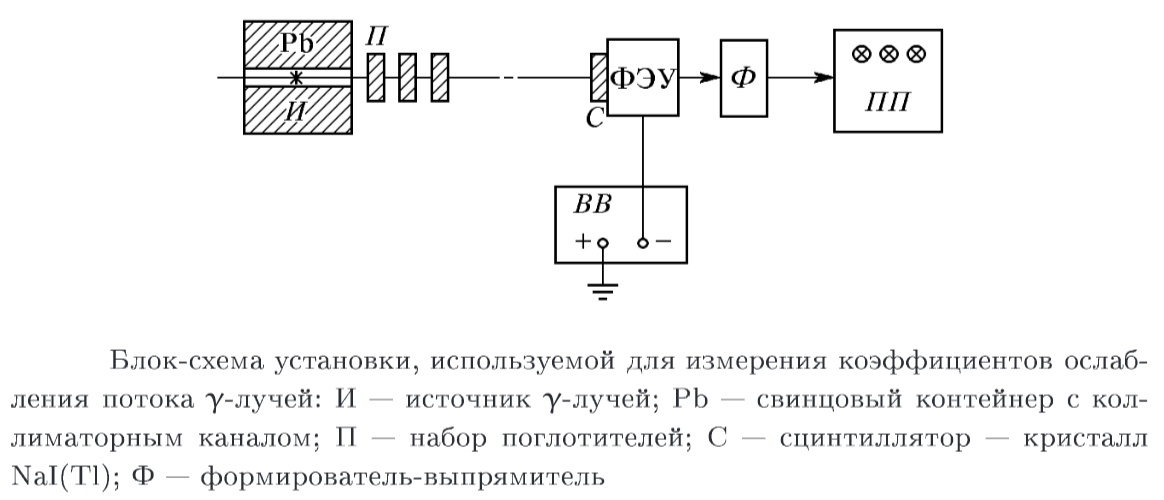
\includegraphics[scale = 0.8]{setup1.png}
    \caption{}
    \label{setup1}
    \end{center}
\end{figure}

\begin{figure}[H]
    \begin{center}
    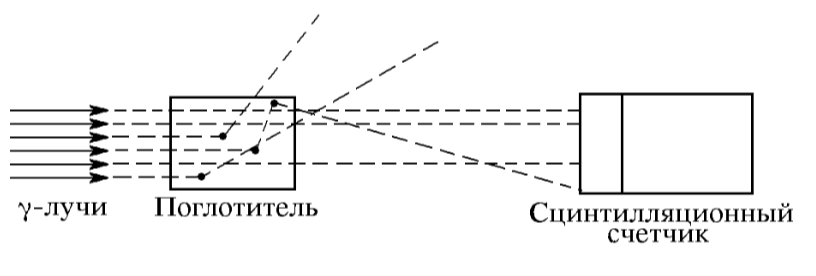
\includegraphics[scale = 0.8]{setup2.png}
    \caption{Схема рассеяния гамма-квантов в поглотителе}
    \label{setup2}
    \end{center}
\end{figure}



\section{Ход работы}

\begin{enumerate}
    \item  Включим пересчетный прибор и высоковольтный выпрямитель. Прогреем их.

    \item Измерим скорость счета фона - со свинцовой пробкой и без, она резко увеличилась как только убрали свинцовую пробку.Получили:
    
    \begin{table}[H]
        \begin{center}
        \begin{tabular}{|l|l|l|}
        \hline
        N, частиц & t, c & I, частиц/c \\ \hline
        3011      & 300  & 10,04       \\ \hline
        \end{tabular}
        \end{center}
        \end{table}

   


    \item Исследуем поглощение гамма-лучей в свинце, железе и алюминии, данные занесем в таблицы ($\sigma_{l_i} = 0,01 см$, $ \sigma_N = \sqrt{N}$):
    
    \item В опыте со свинцом также использовались пробки, изучим ее коэффициент поглощения:
    
    \begin{table}[H]
        \begin{center}
        \begin{tabular}{|l|l|l|l|l|l|}
        \hline
        $l_i$, см & N, частиц & $N_0$, частиц & t, c & I, частиц/c & $I_0$, частиц/c \\ \hline
        2,98     & 459171    & 552550       & 30   & 15305,70    & 18418,33       \\ \hline
        \end{tabular}
        \end{center}
        \end{table}
    
        Рассчитаем $\mu$ ($t_0 = t = 30 с$): 
         \begin{equation}
             \mu = \frac{1}{l}ln\frac{N_0}{N} = 0,06 \pm 0,001 см^{-1}
         \end{equation}
         \begin{equation}
            \sigma_{\mu} = \sqrt{(\frac{\partial \mu}{\partial l})^2\sigma_l^2+(\frac{\partial \mu}{\partial N_0})^2\sigma_{N_0}^2+ (\frac{\partial \mu}{\partial N})^2\sigma_N^2}
        \end{equation}

    \item Эксперимент со свинцом:

    \begin{table}[H]
        \begin{center}
            \begin{tabular}{|l|l|l|l|l|l|l|l|}
                \hline
                Свинец & N, частиц & $N_{без пробки}$, частиц & N-Nф, частиц & I, частиц/c & t, c & $l_i$, см & suml, см \\ \hline
                1      & 514602    & 514602               & 511591       & 17053,03    & 30   & 0        & 0,00     \\ \hline
                2      & 251853    & 251853               & 248842       & 8294,73     & 30   & 0,45     & 0,45     \\ \hline
                3      & 126653    & 151449               & 148438       & 4947,94     & 30   & 0,49     & 0,94     \\ \hline
                4      & 111737    & 111737               & 108726       & 2174,52     & 50   & 0,48     & 1,42     \\ \hline
                5      & 85794     & 102591               & 99580        & 1422,57     & 70   & 0,47     & 1,89     \\ \hline
                6      & 76647     & 76647                & 73636        & 669,42      & 110  & 0,47     & 2,36     \\ \hline
                7      & 68546     & 81966                & 78955        & 464,44      & 170  & 0,49     & 2,85     \\ \hline
                8      & 46761     & 46761                & 43750        & 218,75      & 200  & 0,5      & 3,35     \\ \hline
                9      & 40369     & 48273                & 45262        & 150,87      & 300  & 0,5      & 3,85     \\ \hline
                10     & 26228     & 26228                & 23217        & 77,39       & 300  & 0,5      & 4,35     \\ \hline
            \end{tabular}
            \caption{Свинец}
        \end{center}
    \end{table}

    \begin{figure}[H]
        \begin{center}
        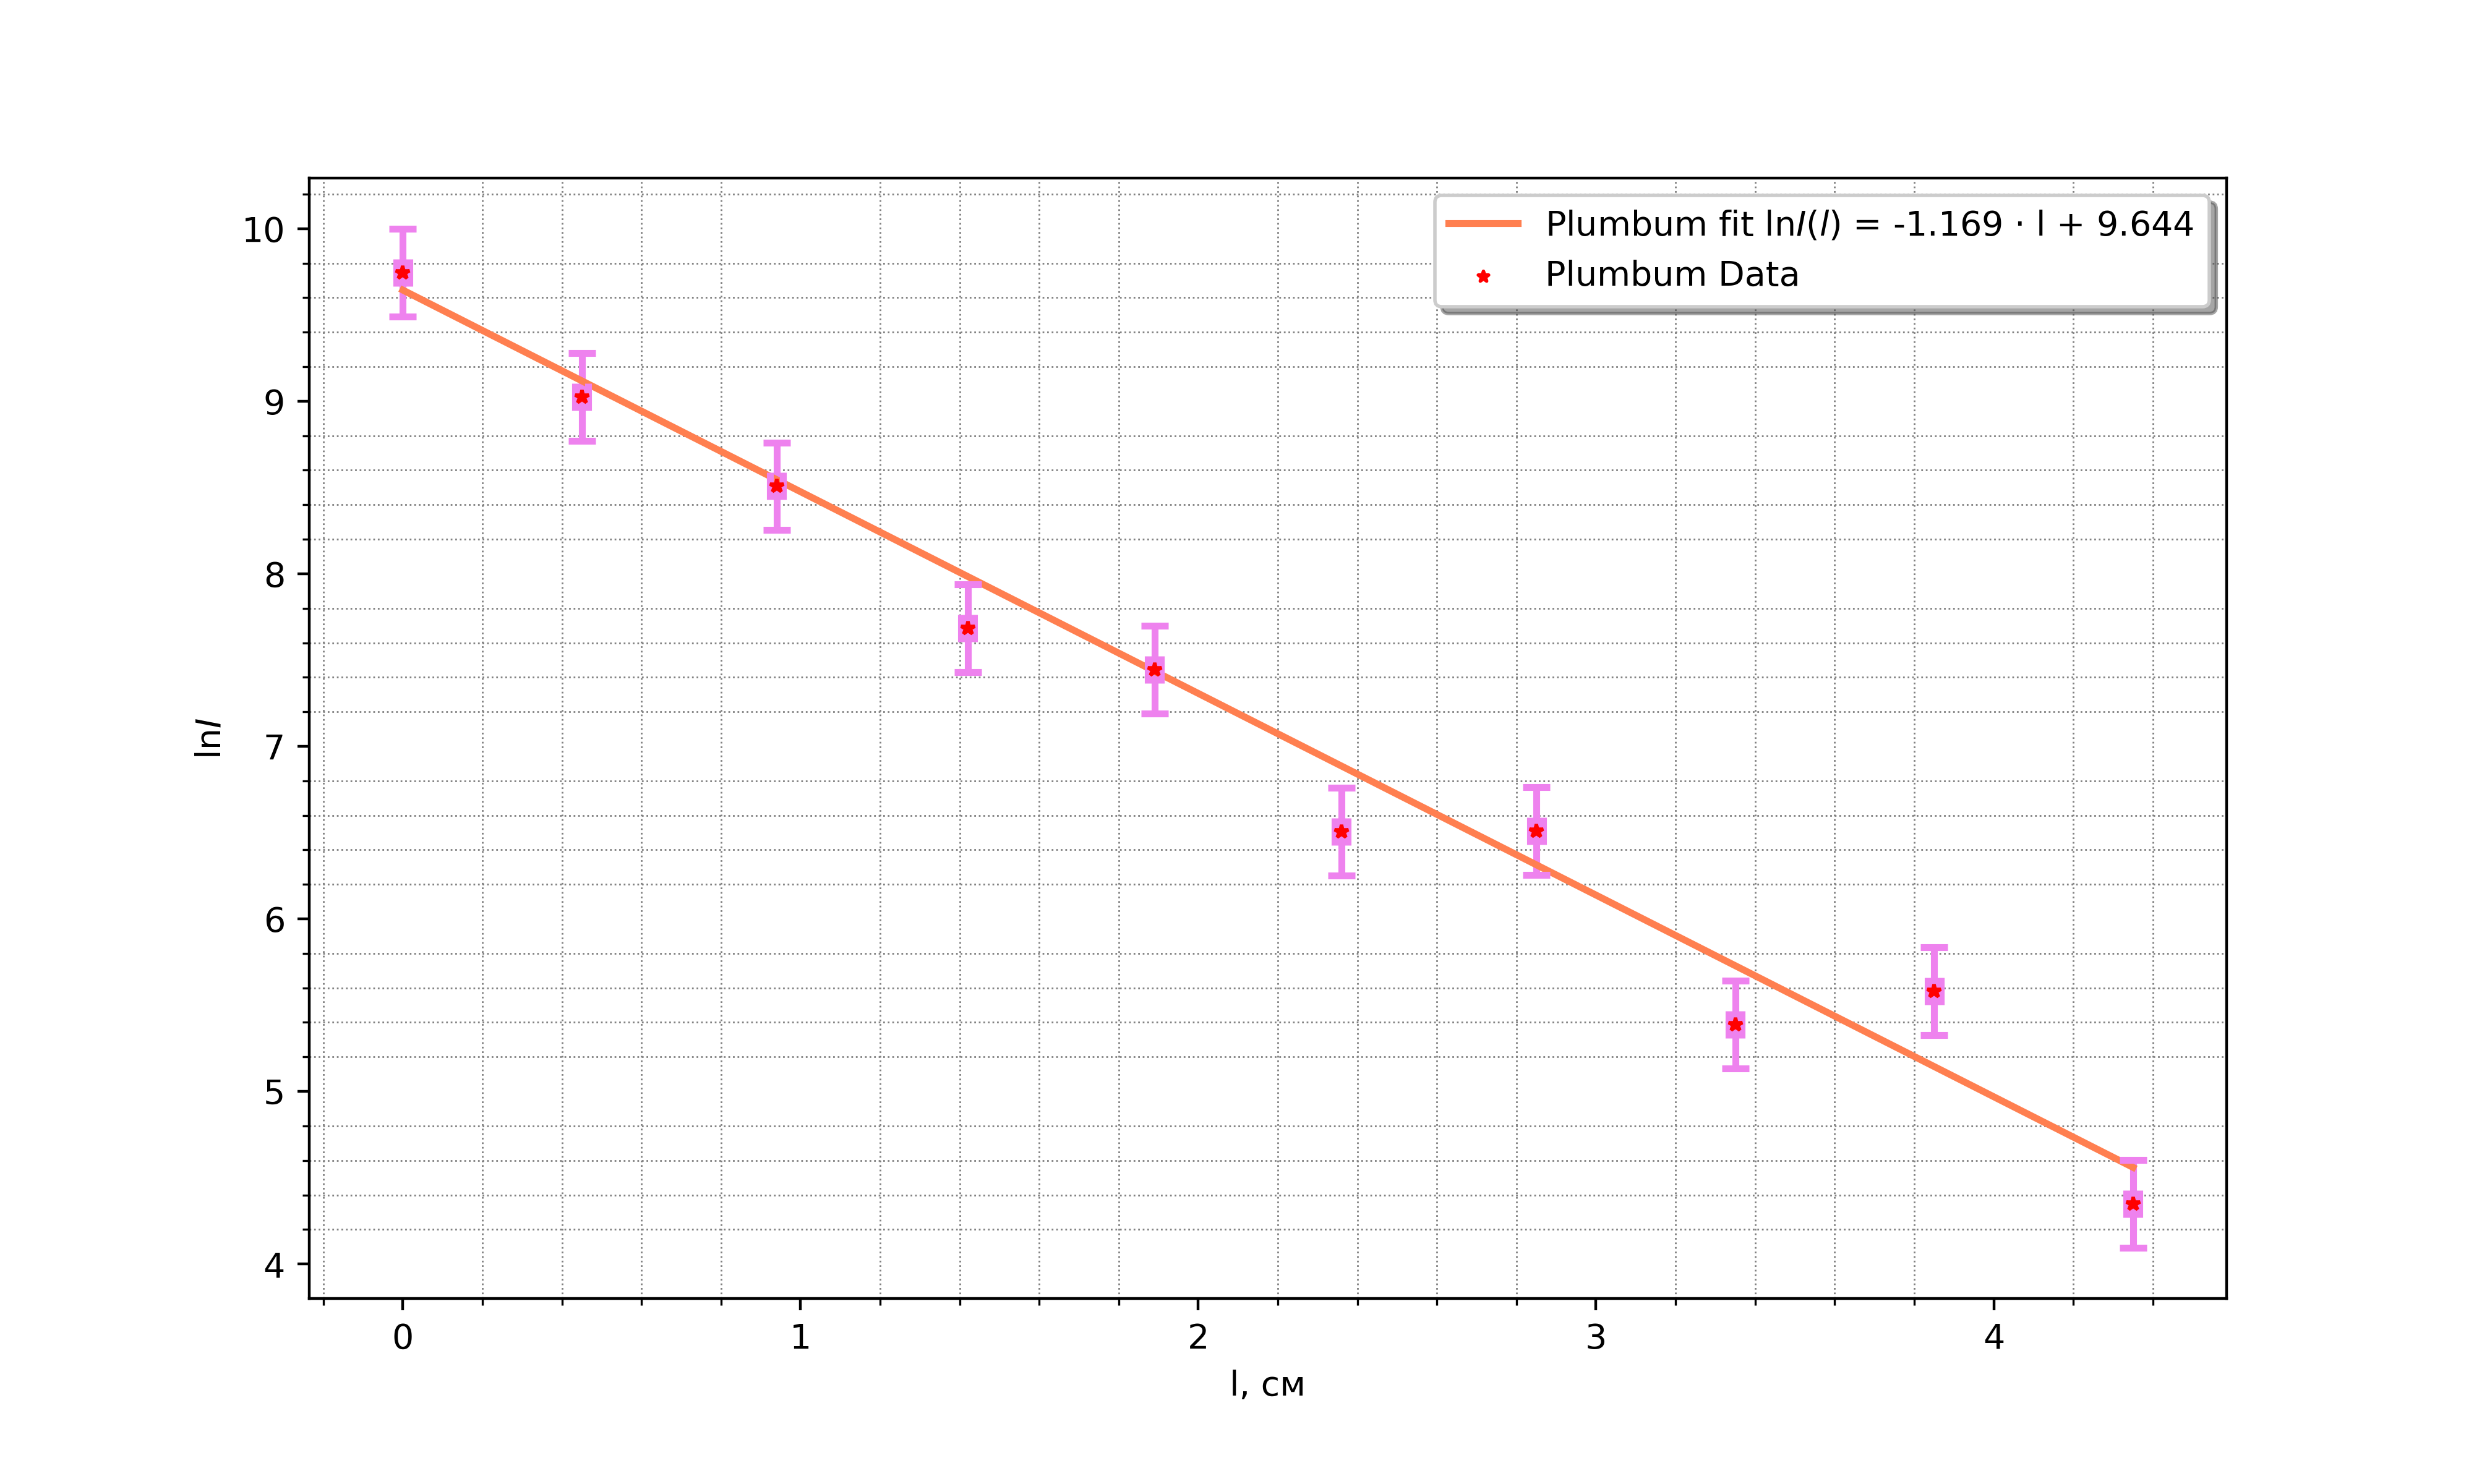
\includegraphics[scale = 0.65]{Pb.png}
        \caption{Зависимость $\ln{I}(l) = \ln{I_0} -  l\cdot \mu $ для свинца}
        \label{Pb}
        \end{center}
    \end{figure}

    \item Эксперимент с алюминием:
        \begin{table}[H]
            \begin{center}
                \begin{tabular}{|l|l|l|l|l|l|l|}
                    \hline
                    Алюминий & N, частиц & N-Nф, частиц & I, частиц/c & t, c &  $l_i$, см & suml, см \\ \hline
                    1        & 550330    & 547319       & 18243,97    & 30   & 0,00     & 0,00     \\ \hline
                    2        & 420498    & 417487       & 10437,18    & 40   & 1,97     & 1,97     \\ \hline
                    3        & 250709    & 247698       & 6192,45     & 40   & 2,00     & 3,97     \\ \hline
                    4        & 235649    & 232638       & 3877,30     & 60   & 2,00     & 5,97     \\ \hline
                    5        & 148731    & 145720       & 2428,67     & 60   & 1,99     & 7,96     \\ \hline
                    6        & 113508    & 110497       & 1578,53     & 70   & 2,00     & 9,96     \\ \hline
                    7        & 96376     & 93365        & 1037,39     & 90   & 1,97     & 11,93    \\ \hline
                    8        & 70860     & 67849        & 678,49      & 100  & 2,01     & 13,94    \\ \hline
                    9        & 47409     & 44398        & 443,98      & 100  & 2,01     & 15,95    \\ \hline
                    10       & 35228     & 32217        & 322,17      & 100  & 2,00     & 17,95    \\ \hline
                \end{tabular}
            \caption{Алюминий}
            \end{center}
        \end{table}

        \begin{figure}[H]
            \begin{center}
            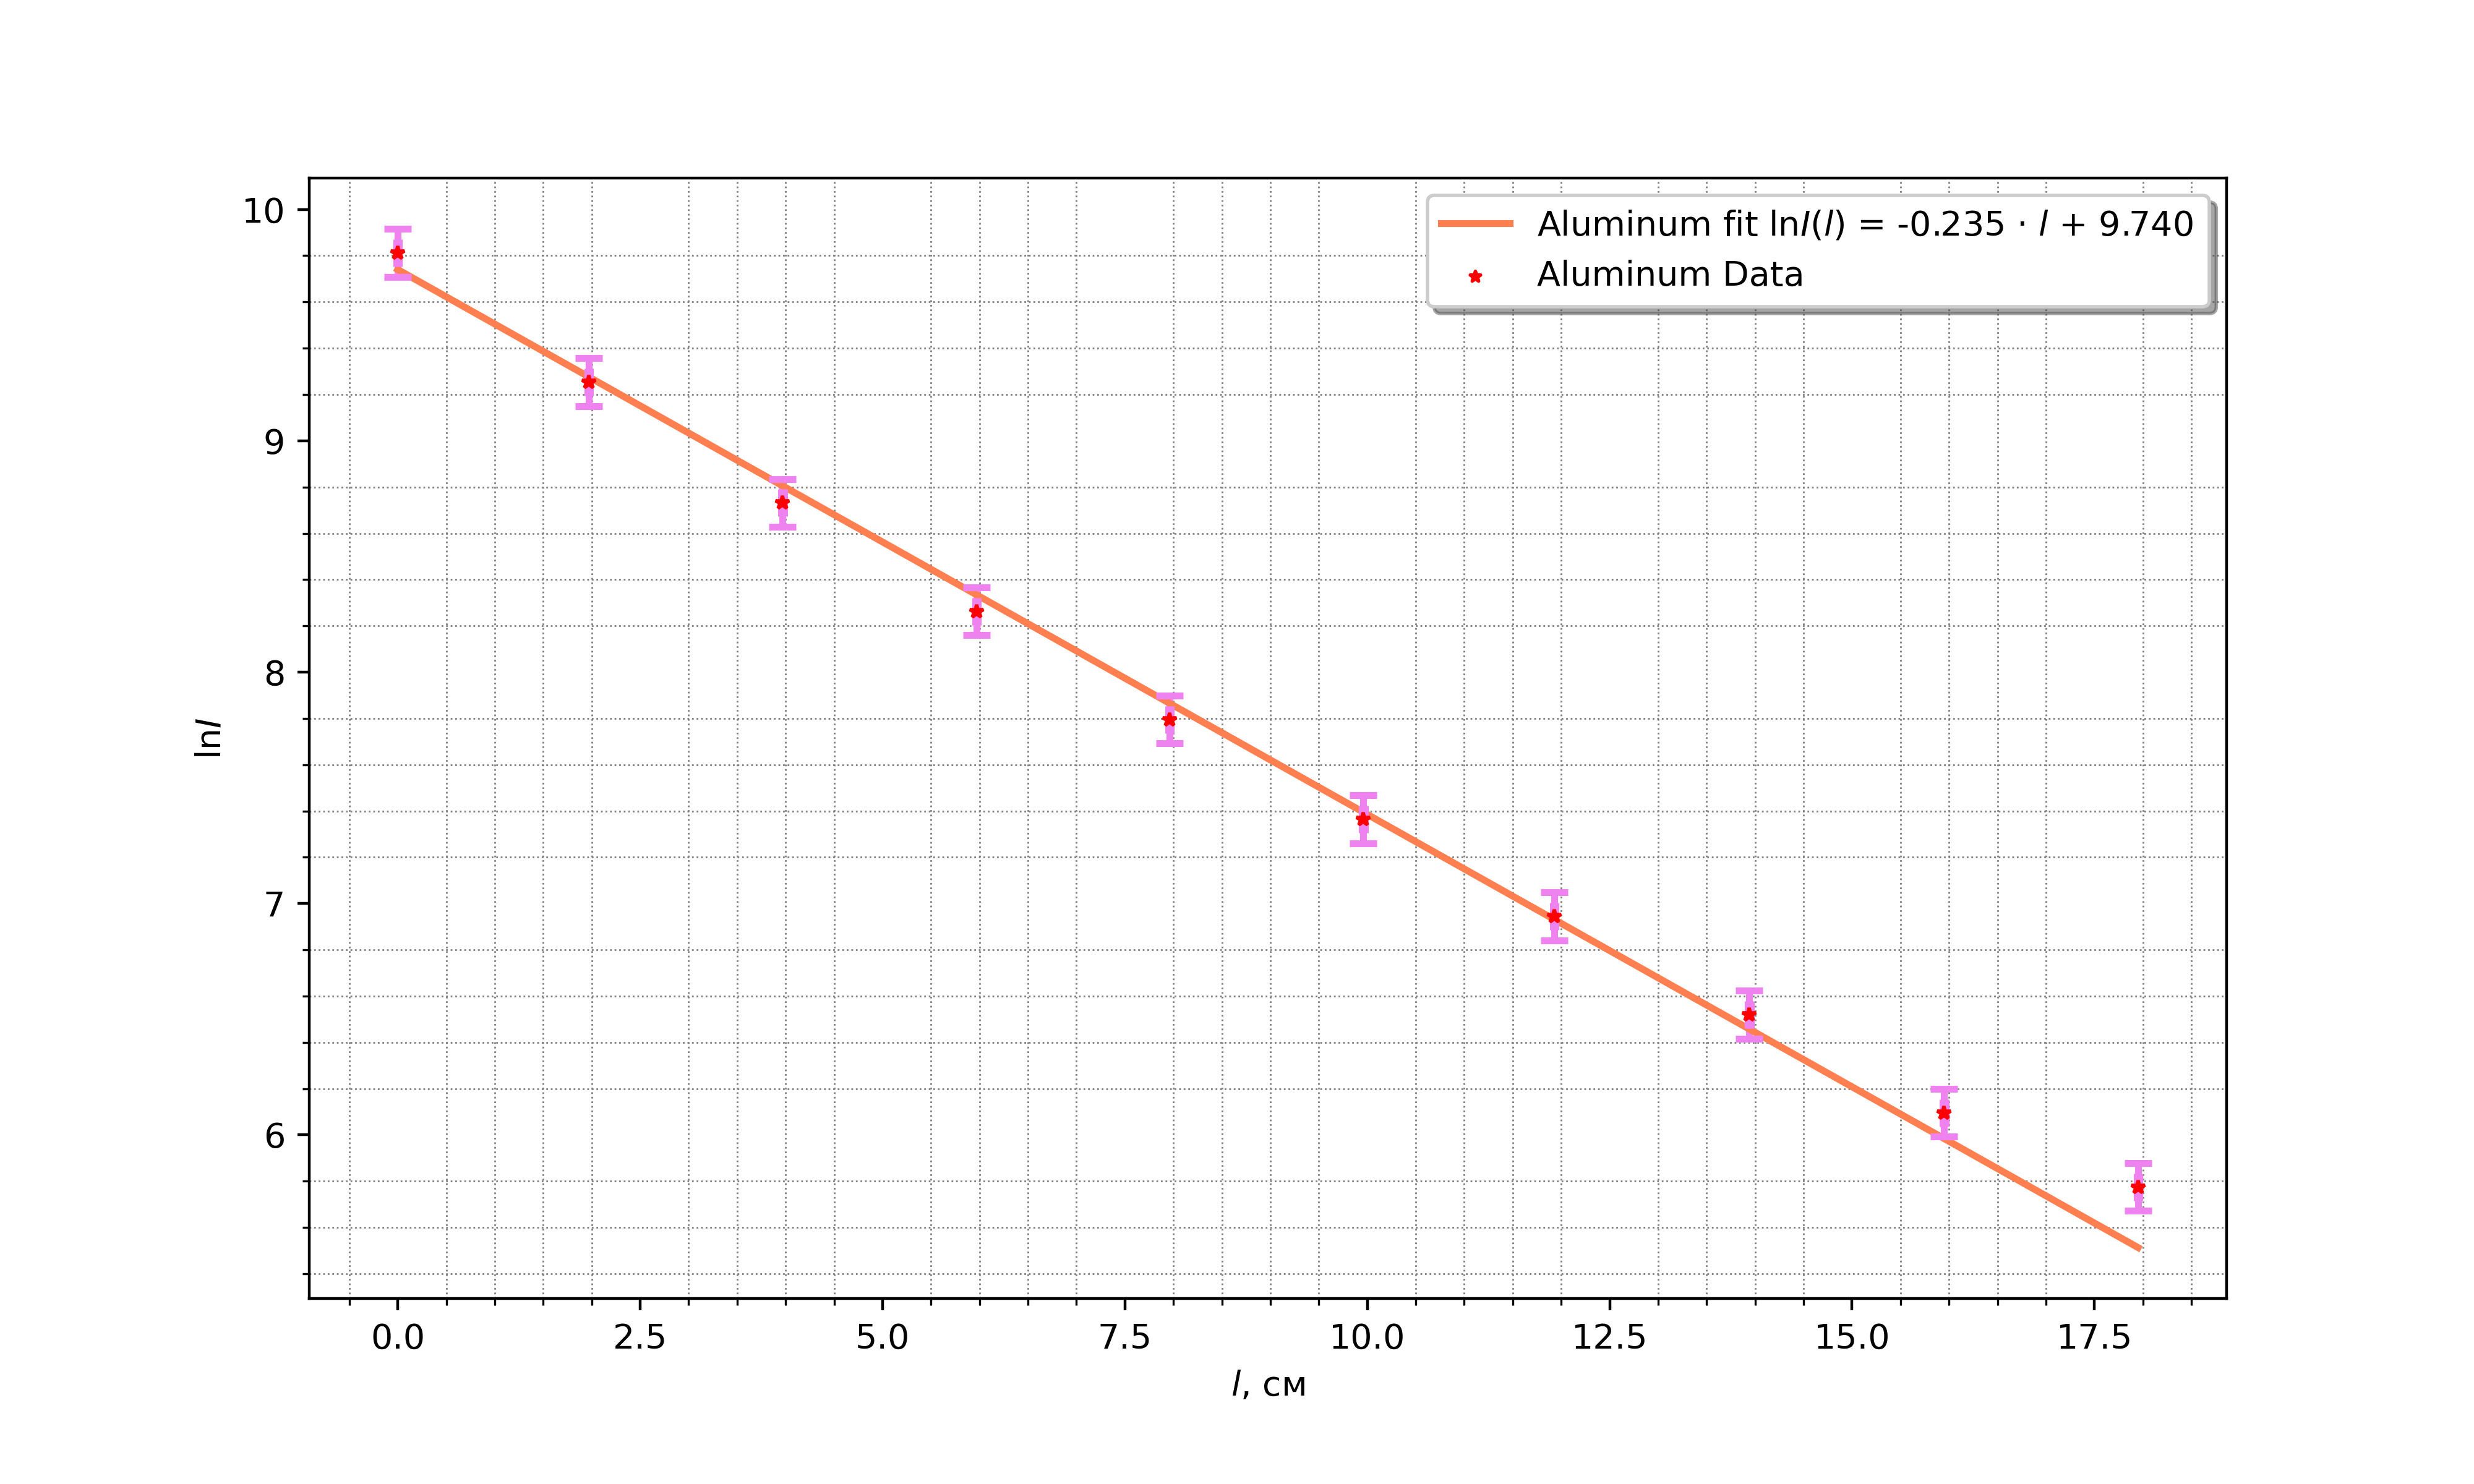
\includegraphics[scale = 0.65]{Al.png}
            \caption{Зависимость $\ln{I}(l) = \ln{I_0} -  l\cdot \mu $ для алюминия}
            \label{Al}
            \end{center}
        \end{figure}

    \item Эксперимент с железом:
        \begin{table}[H]
            \begin{center}
                \begin{tabular}{|l|l|l|l|l|l|l|}
                    \hline
                    Железо & N, частиц & N-Nф, частиц & I, частиц/c & t, c &  $l_i$, см & suml, см \\ \hline
                    1      & 7466706   & 7463695      & 186667,65   & 40   & 0,00     & 0,00     \\ \hline
                    2      & 265900    & 262889       & 8863,33     & 30   & 1,01     & 1,01     \\ \hline
                    3      & 177197    & 174186       & 4429,93     & 40   & 1,01     & 2,02     \\ \hline
                    4      & 117172    & 114161       & 2343,44     & 50   & 1,00     & 3,02     \\ \hline
                    5      & 89284     & 86273        & 1275,49     & 70   & 1,00     & 4,02     \\ \hline
                    6      & 56897     & 53886        & 711,21      & 80   & 1,01     & 5,03     \\ \hline
                    7      & 39823     & 36812        & 398,23      & 100  & 1,01     & 6,04     \\ \hline
                    8      & 28317     & 25306        & 235,98      & 120  & 1,02     & 7,06     \\ \hline
                    9      & 20887     & 17876        & 139,25      & 150  & 1,00     & 8,06     \\ \hline
                    10     & 20485     & 17474        & 85,35       & 240  & 1,03     & 9,09     \\ \hline
                \end{tabular}
            \caption{Железо}
            \end{center}
        \end{table}
            
        \begin{figure}[H]
            \begin{center}
            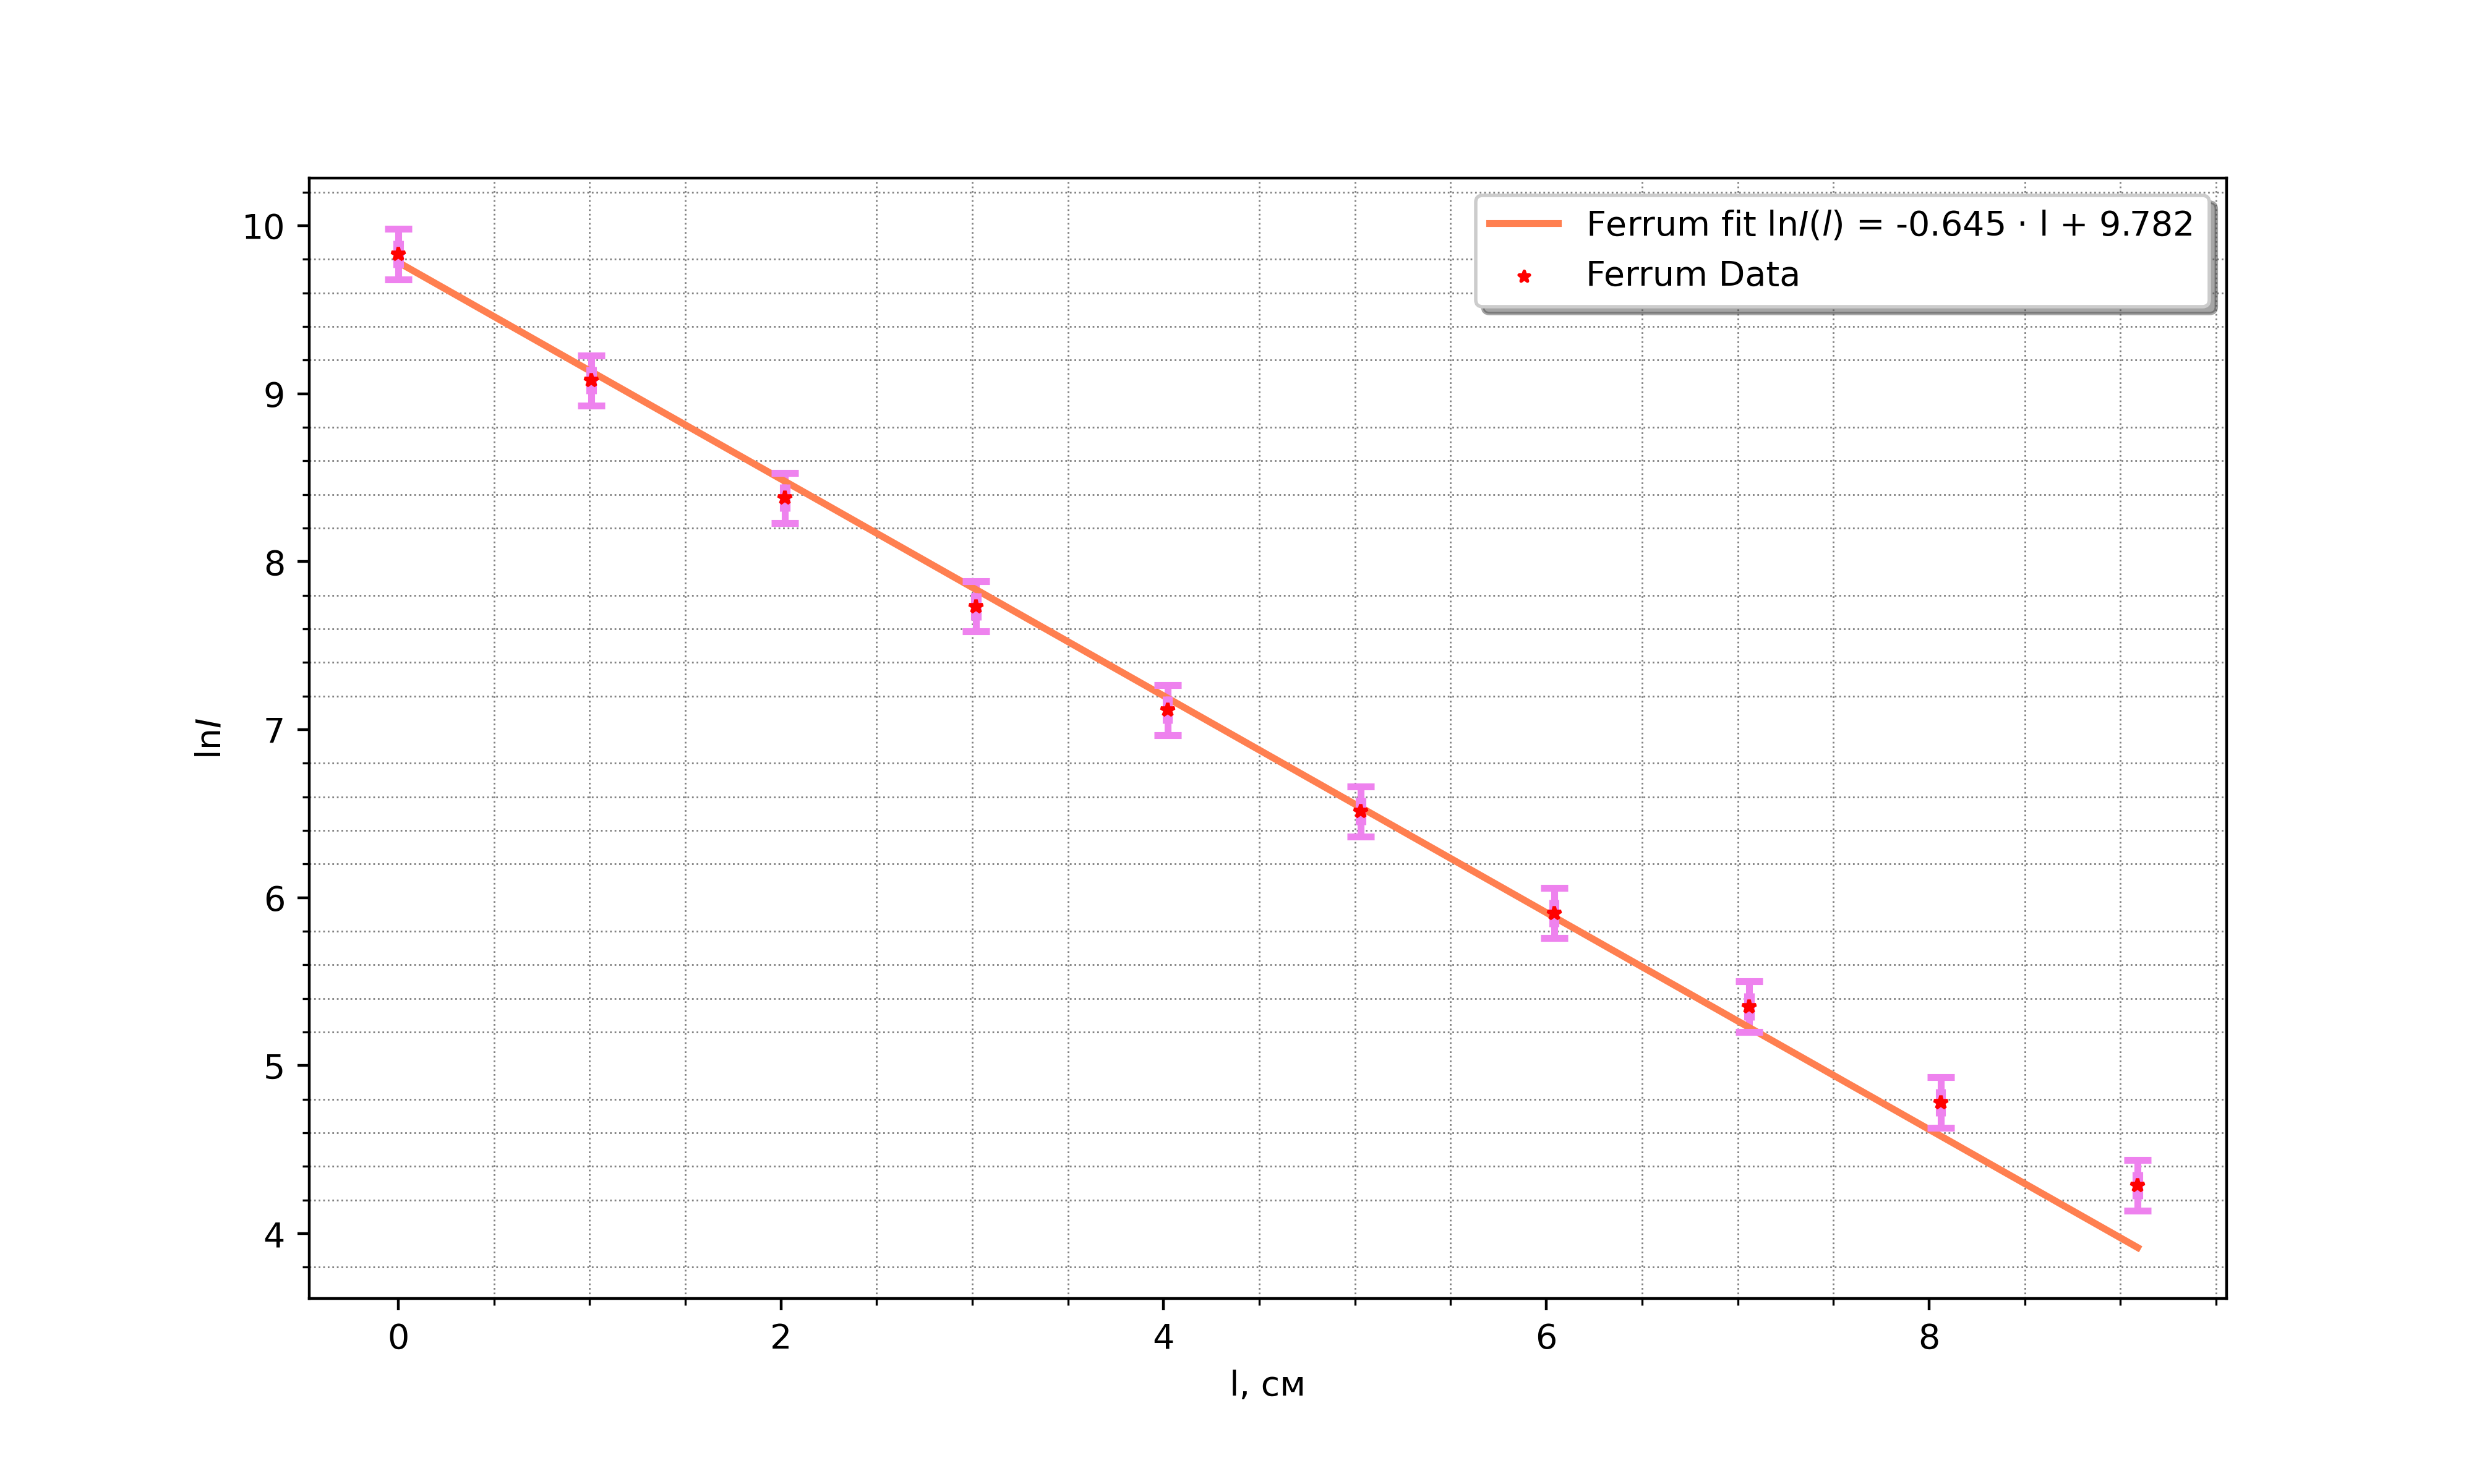
\includegraphics[scale = 0.65]{Fe.png}
            \caption{Зависимость $\ln{I}(l) = \ln{I_0} -  l\cdot \mu $ для железа}
            \label{Fe}
            \end{center}
        \end{figure}
    

    \item Для каждого вида поглотителей построим зависимость $\ln{N}(l) = \ln{N_0} -  l\cdot \mu $
    на рис. \ref{Al}, \ref{Pb}, \ref{Fe}:

    Откуда получим линейный коэффициент $\mu$ как тангенс угла наклона:

    $$\mu_{Al} = (0.24 \pm 0.01) \; см^{-1}$$
    $$\mu_{Pb} = (1.17 \pm 0.05 )\; см^{-1}$$
    $$\mu_{Fe} = (0.65 \pm 0.01 )\; см^{-1}$$

    По линейным коэффициентам рассчитаем коэффициенты $\mu'$ по ф-ле (1) следует, что:
    $\mu' = \frac{\mu \cdot l}{m_1} = \frac{\mu}{\rho}$
    
    $$\mu'_{Al} = (0.089 \pm 0.004) см^{2}/г, \; \rho_{Al} = 2,70 г/см^3 $$
    $$\mu'_{Pb} = (0.103 \pm 0.004) см^{2}/г, \; \rho_{Pb} = 11,35 г/см^3 $$
    $$\mu'_{Fe} = (0.083 \pm 0.001) см^{2}/г,\; \rho_{Fe} = 7,87 г/см^3 $$


    \item Определим среднюю энерегию гамма-квантов по таблице №1. 
        
        \begin{figure}[H]
            \begin{center}
            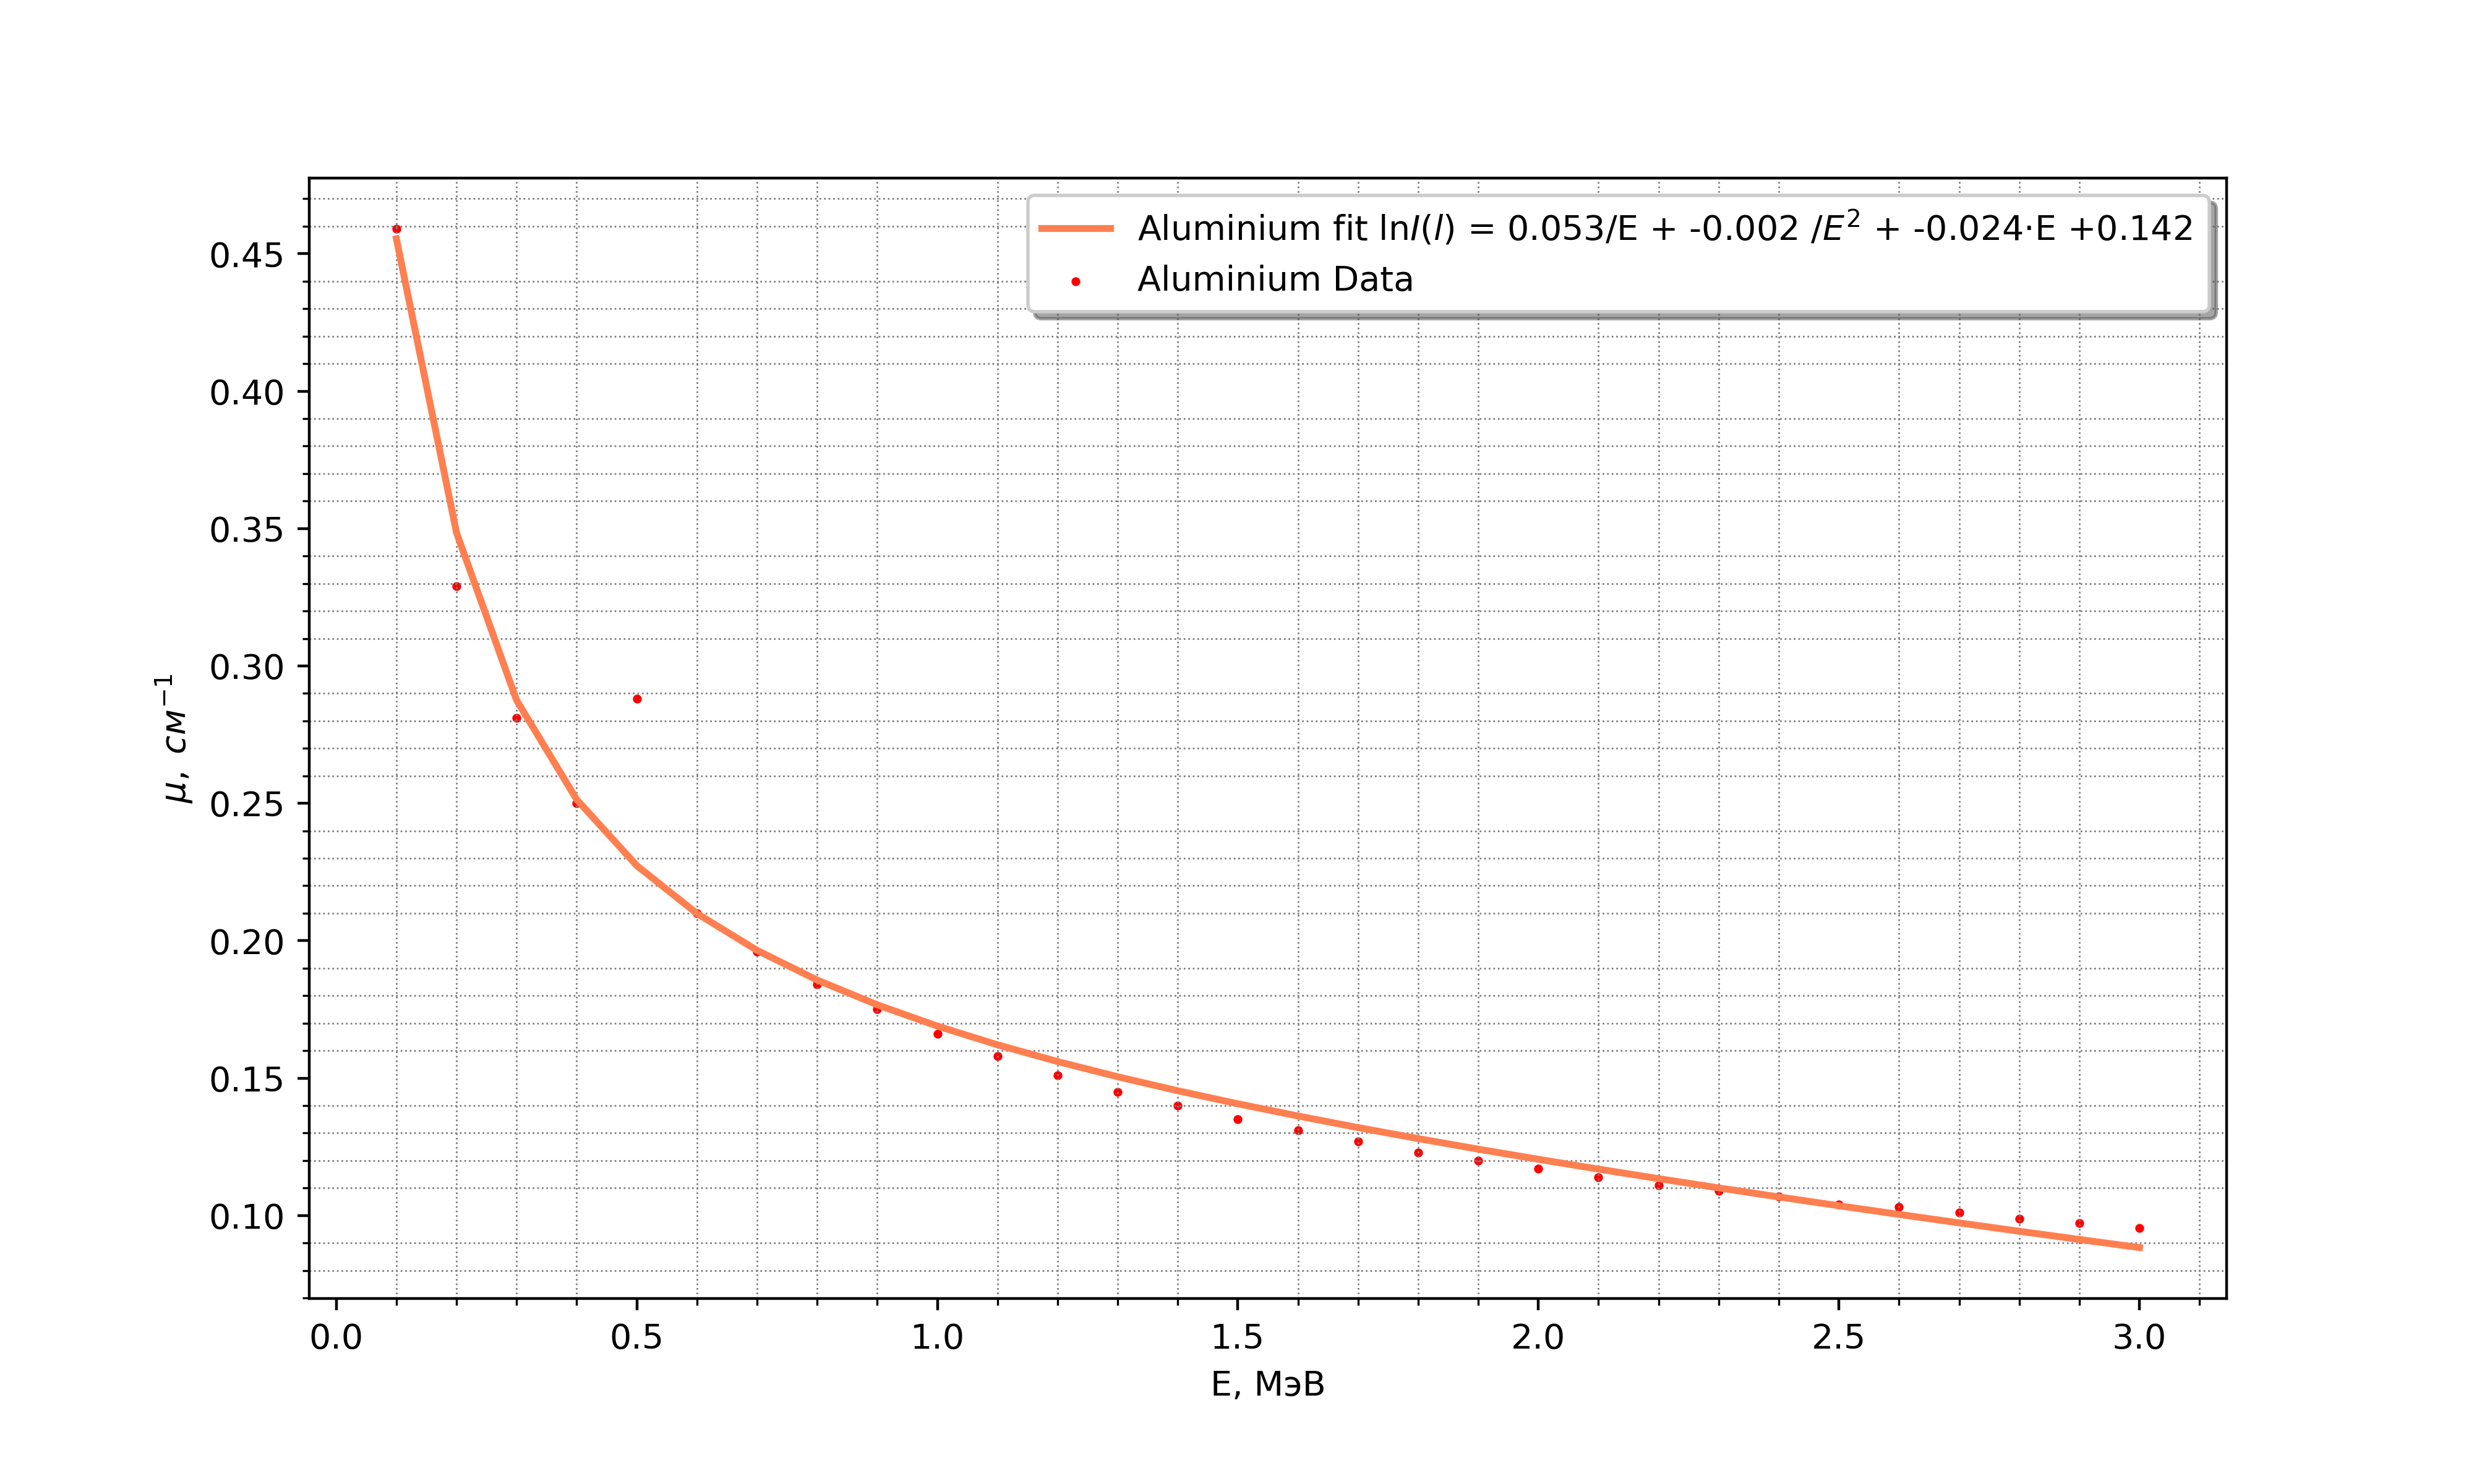
\includegraphics[scale = 0.65]{al_e.png}
            \caption{Зависимость $\mu(E)$ для алюминия}
            \label{Al}
            \end{center}
        \end{figure}

        $${E_{\gamma}} \approx (0.48 \pm 0.05)\; МэВ$$

    \item
        \begin{figure}[H]
            \begin{center}
            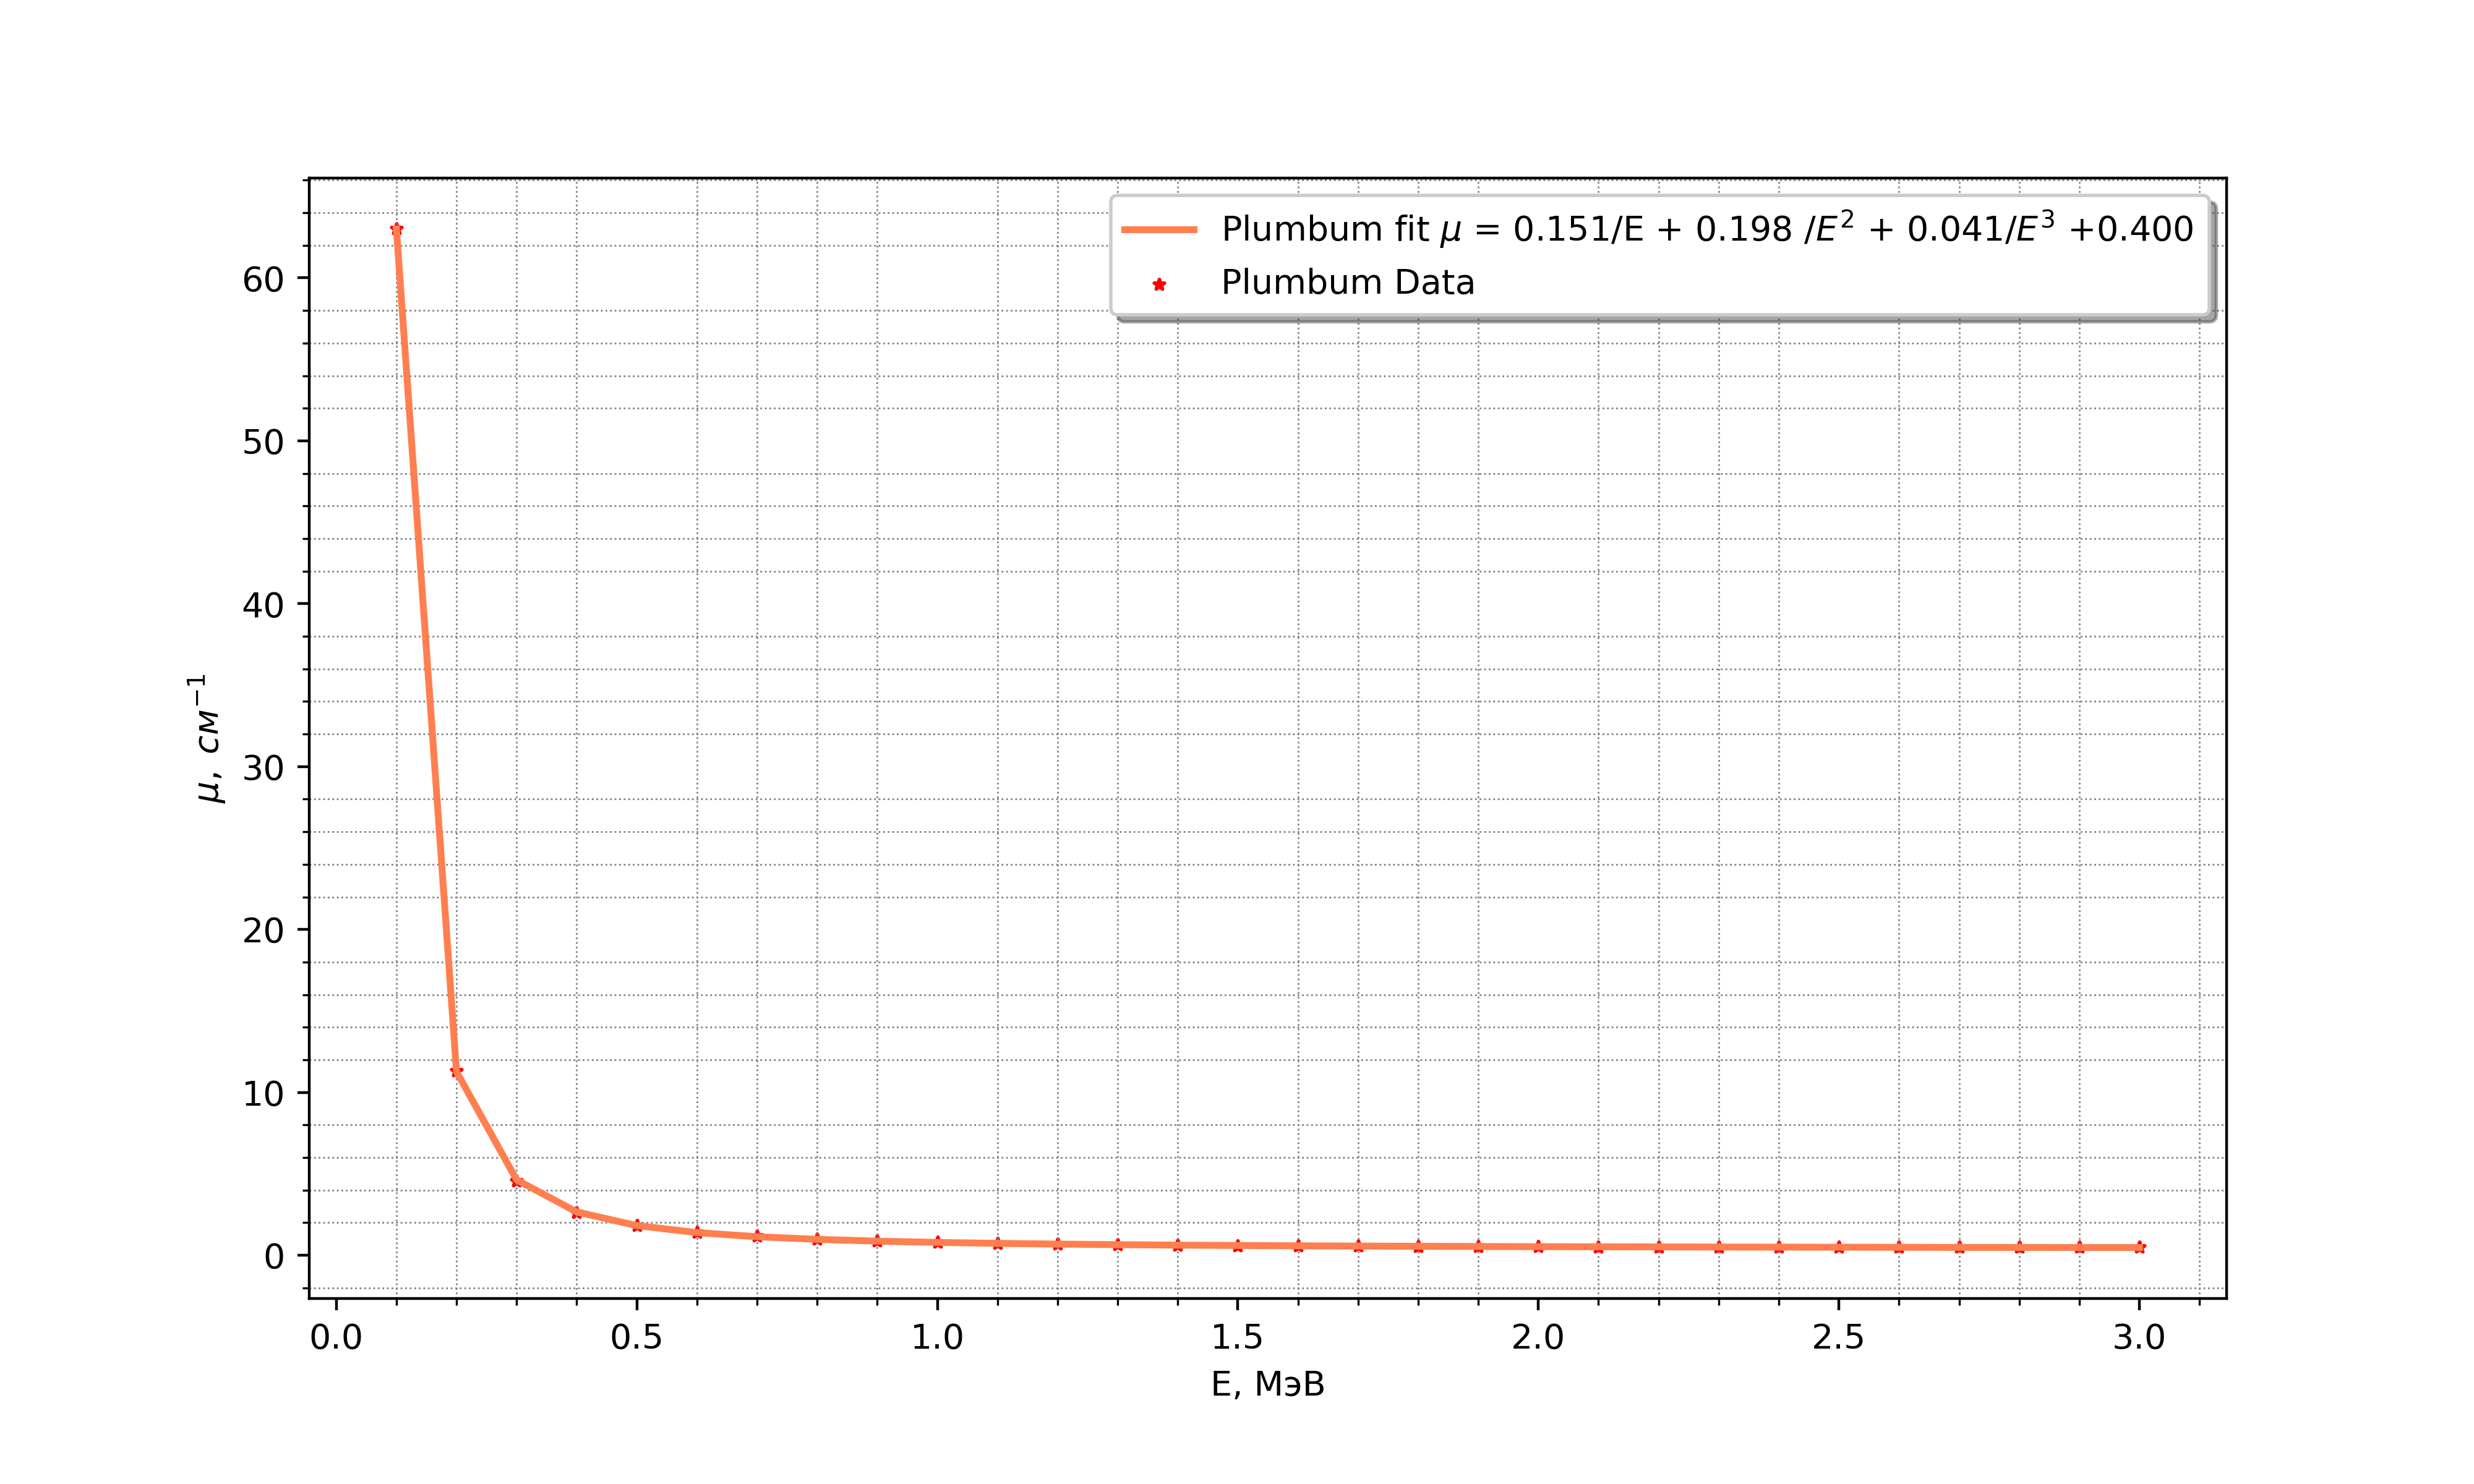
\includegraphics[scale = 0.65]{pb_e.png}
            \caption{Зависимость $\mu(E)$ для свинца}
            \label{Al}
            \end{center}
        \end{figure}

        \begin{figure}[H]
            \begin{center}
            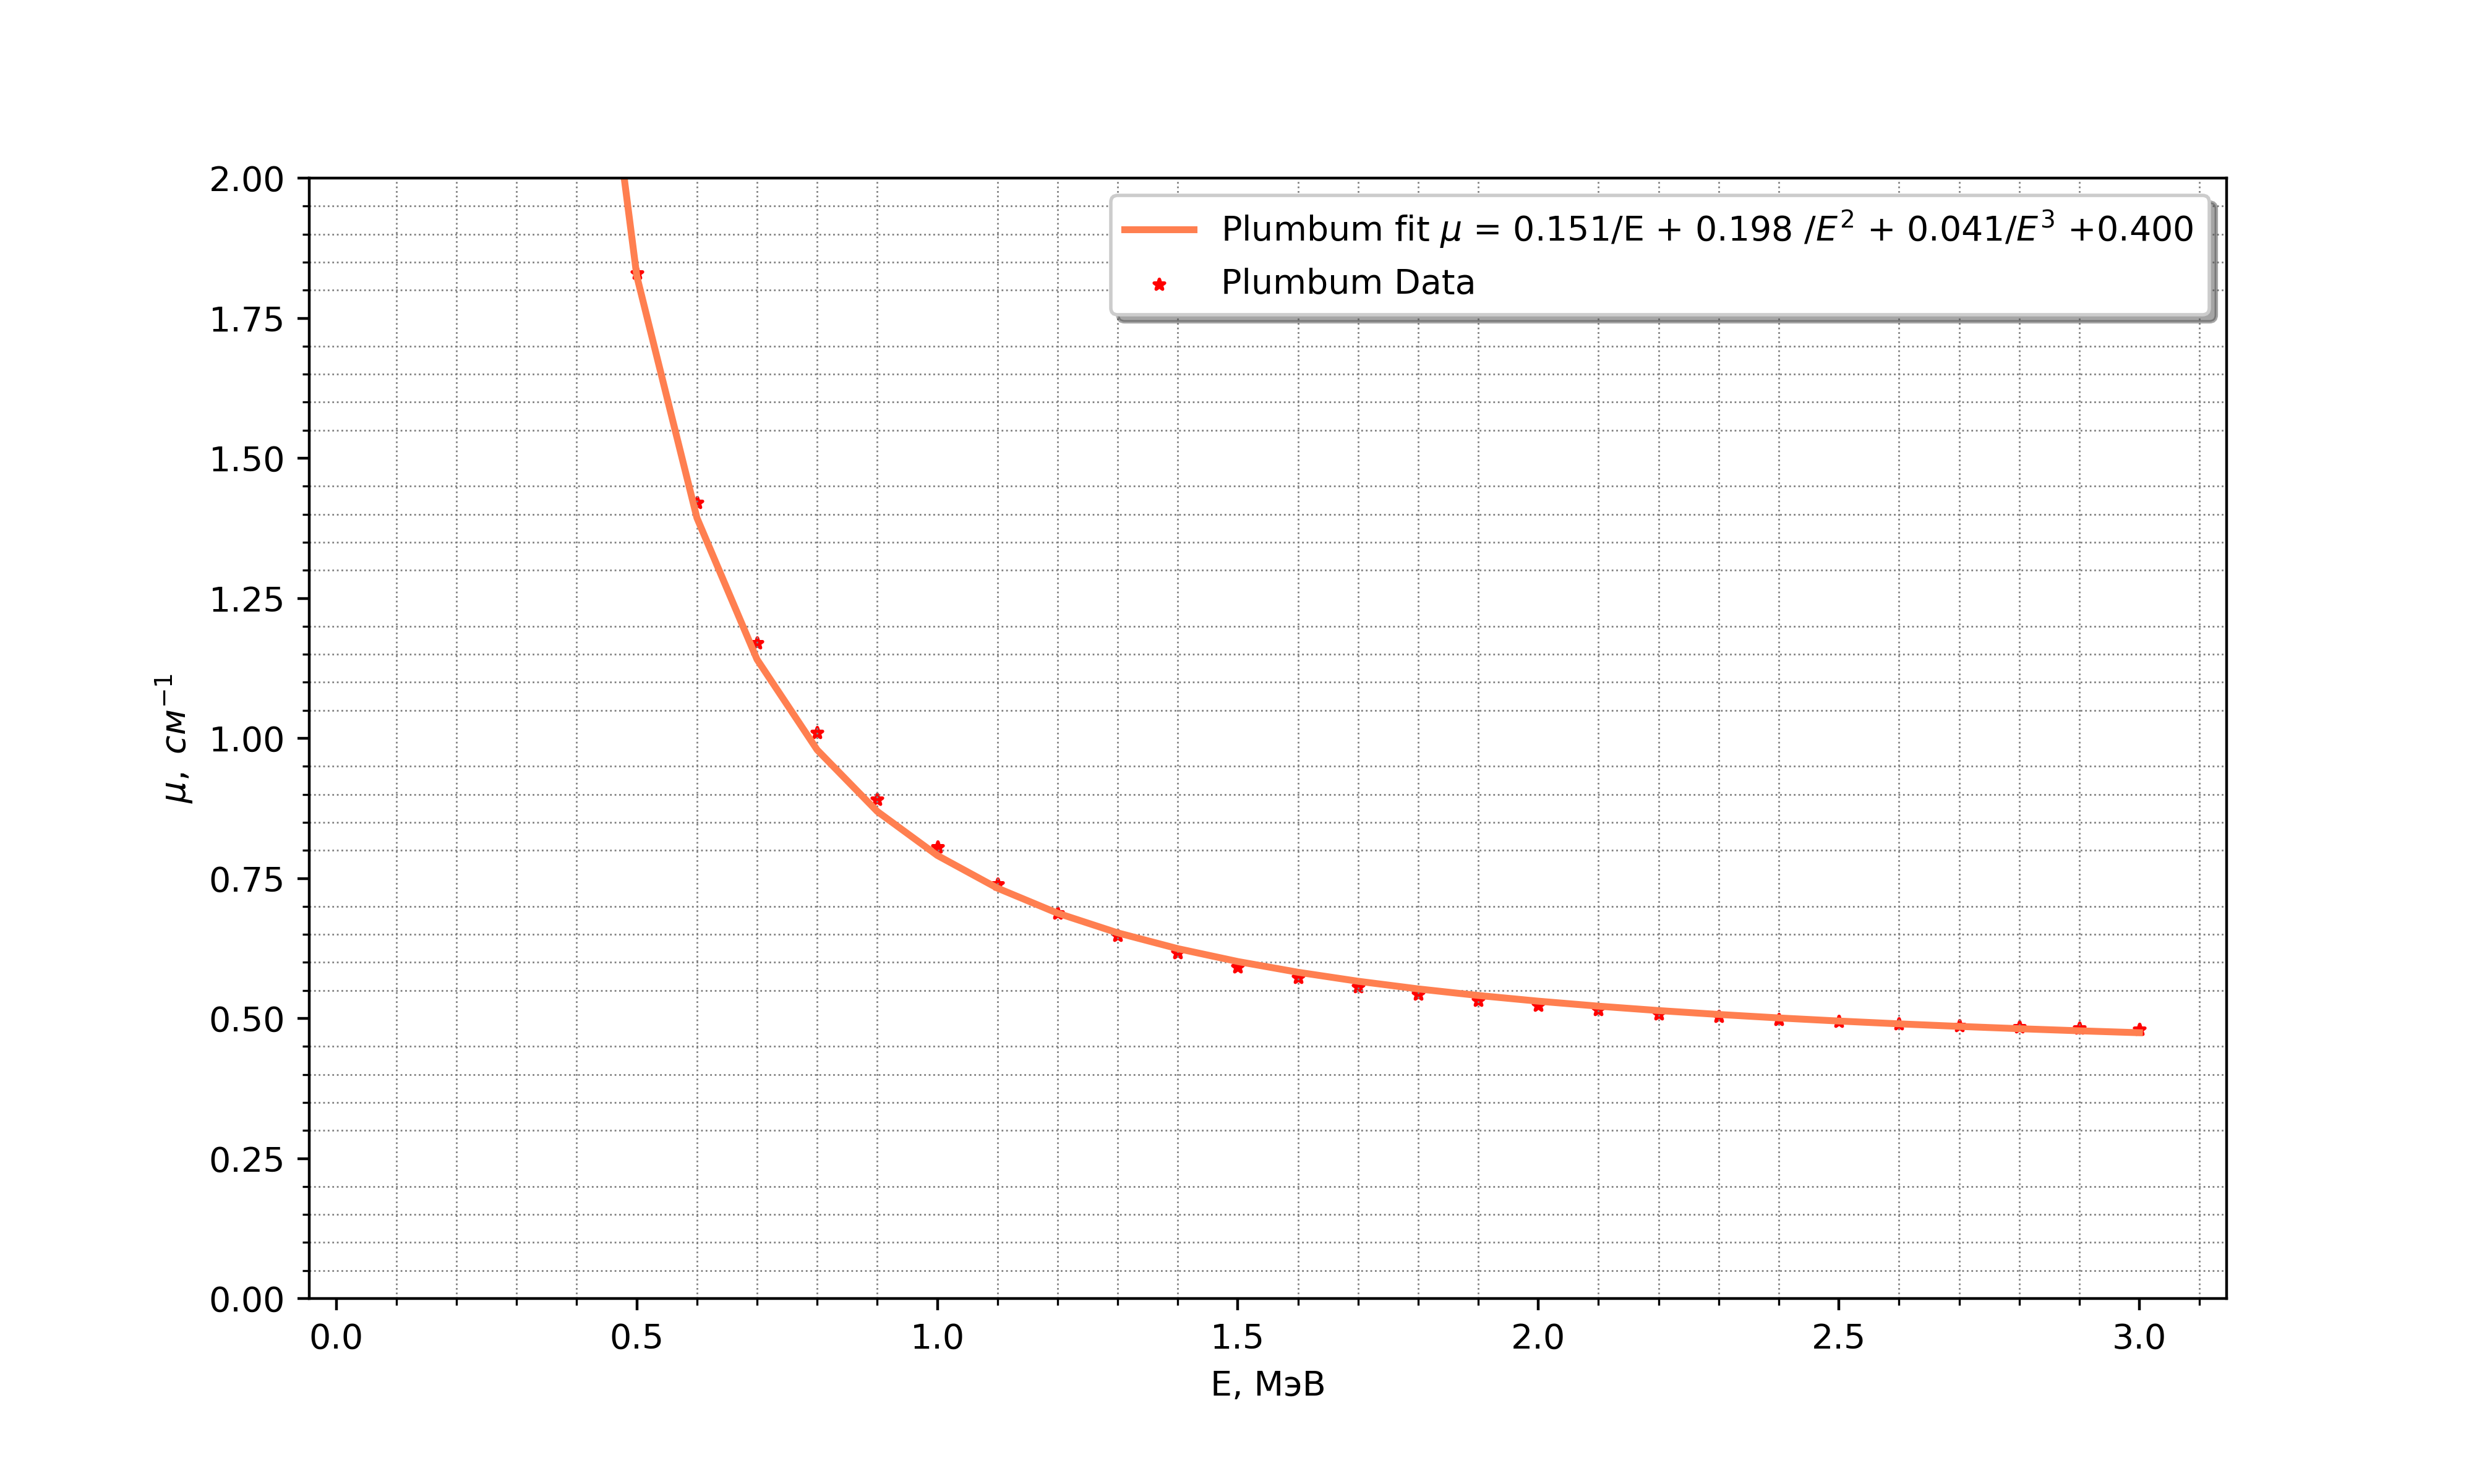
\includegraphics[scale = 0.65]{pb_e2.png}
            \caption{Зависимость $\mu(E)$ для свинца}
            \label{Al}
            \end{center}
        \end{figure}

        $${E_{\gamma}} \approx (0,68 \pm 0,05)\; МэВ$$

    \item
        \begin{figure}[H]
            \begin{center}
            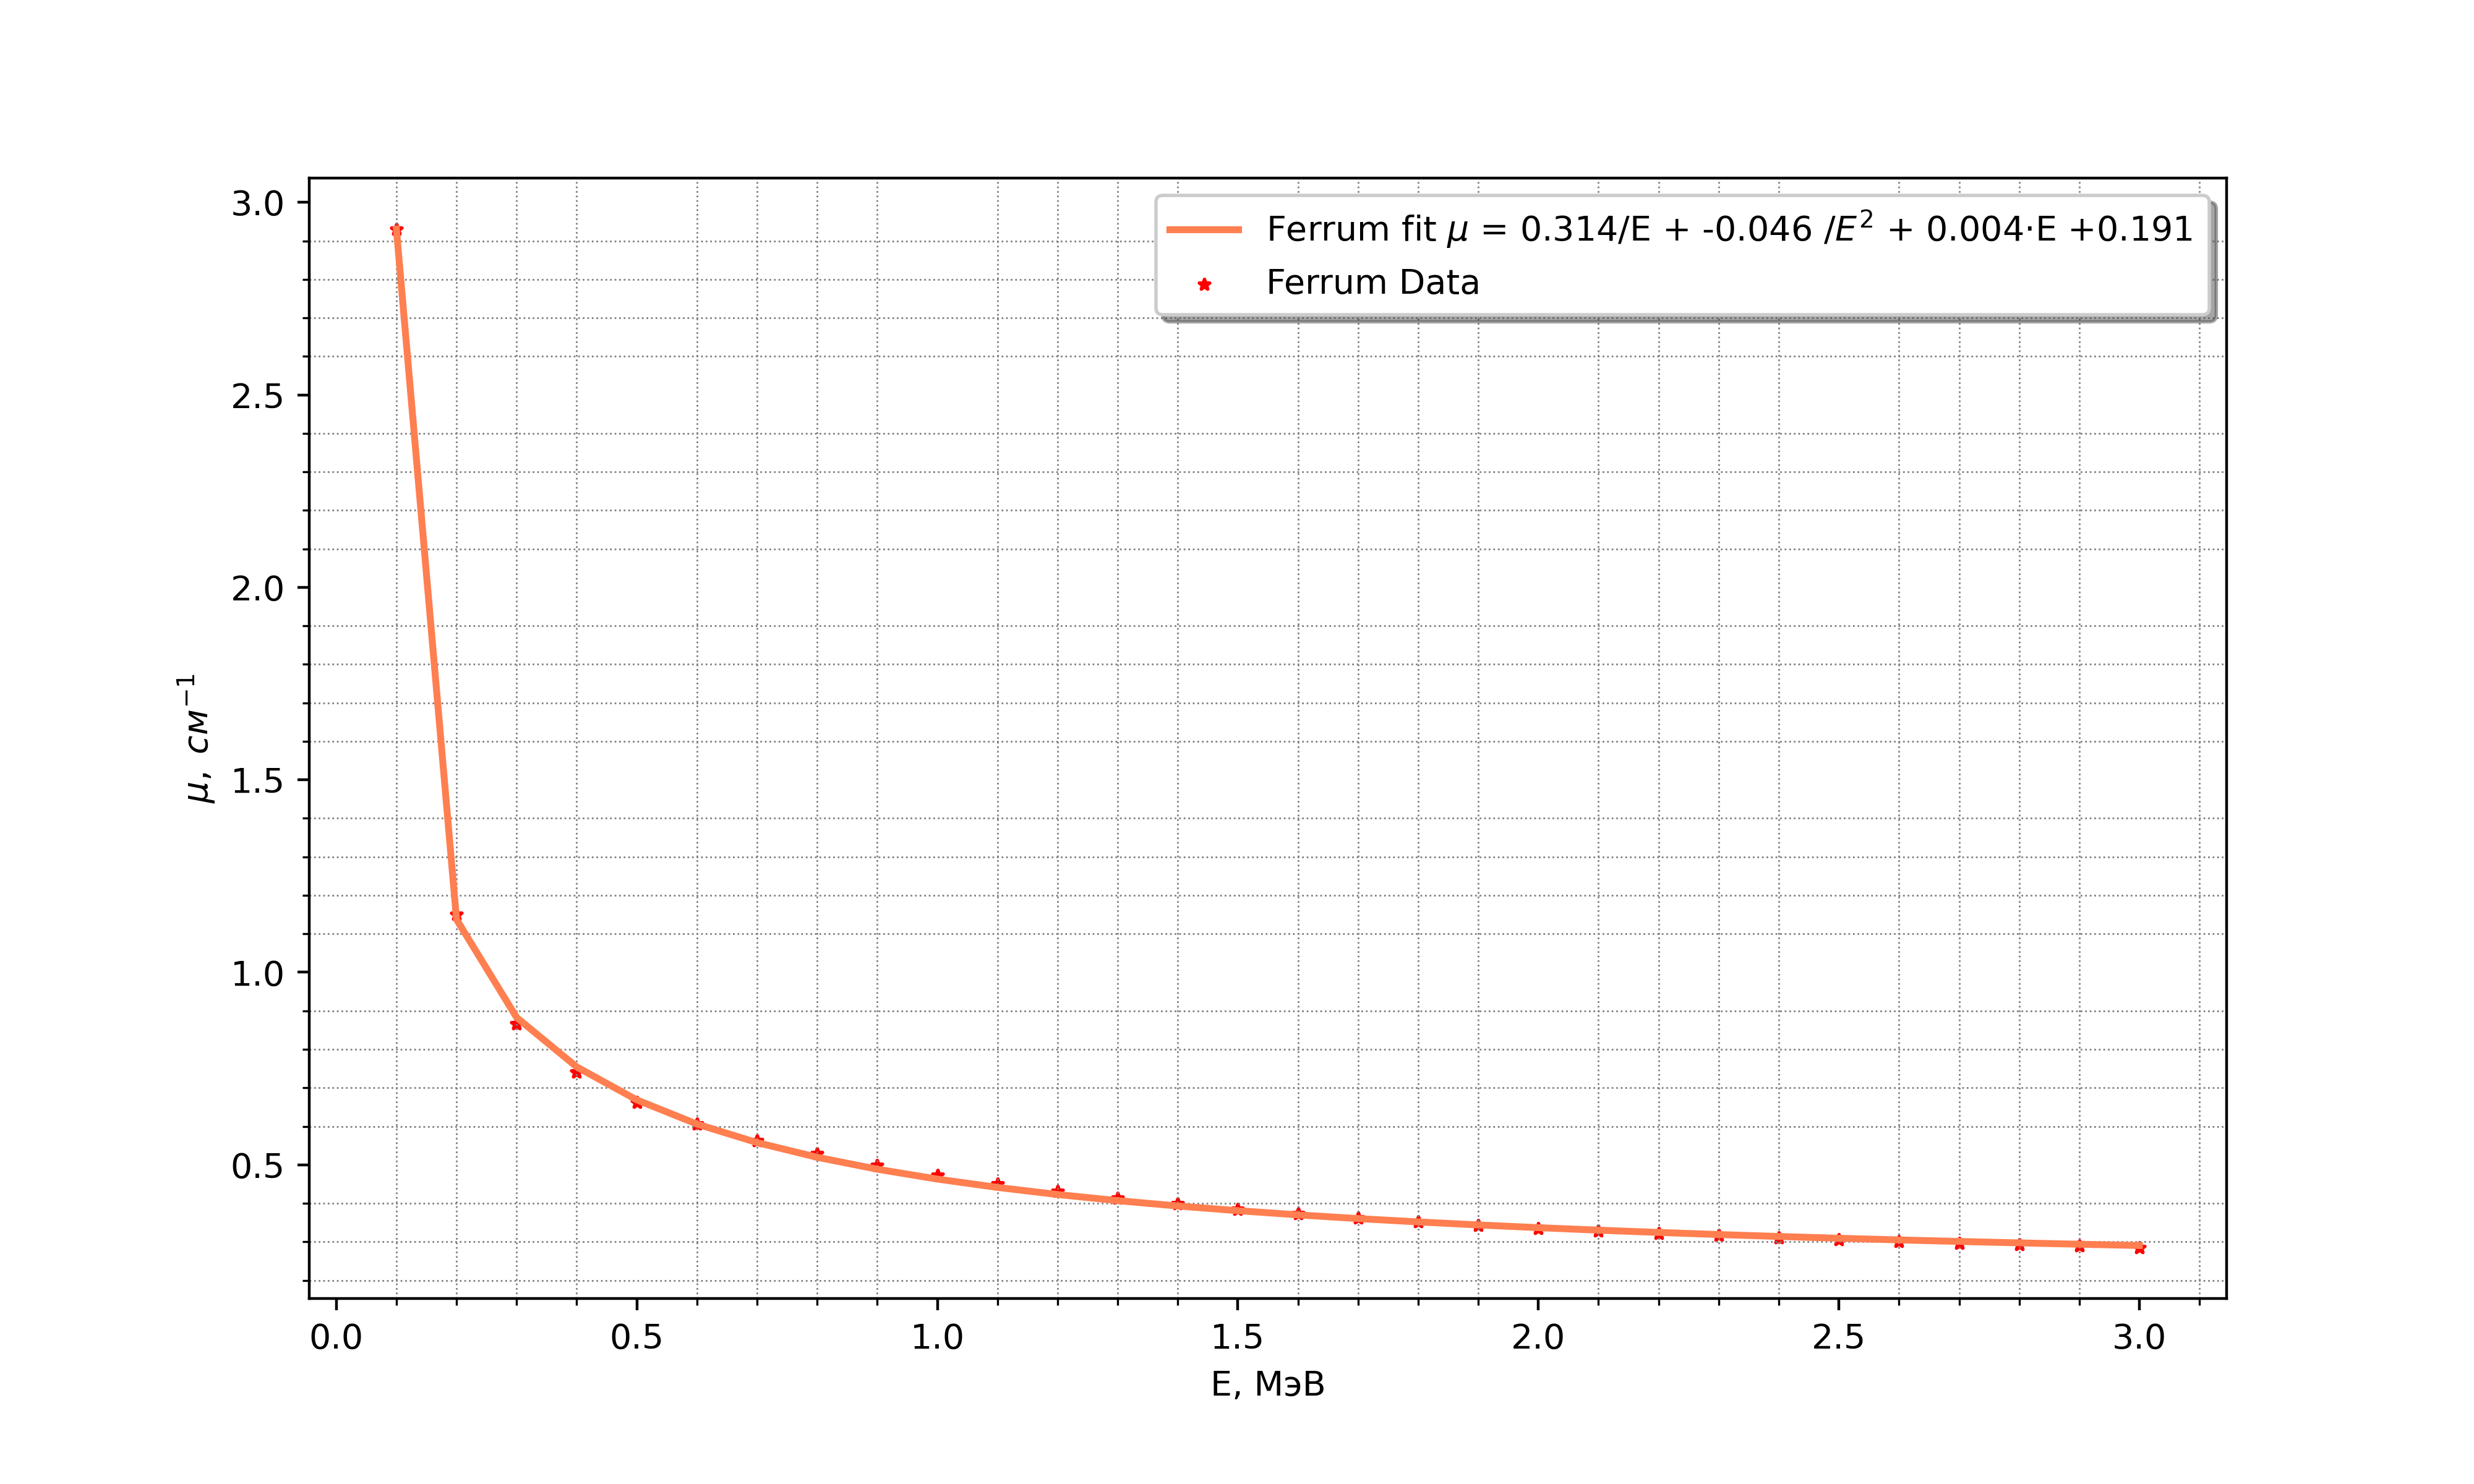
\includegraphics[scale = 0.65]{fe_e.png}
            \caption{Зависимость $\mu(E)$ для железа}
            \label{Al}
            \end{center}
        \end{figure}

        $${E_{\gamma}} \approx (0,50 \pm 0,05)\; МэВ$$

    \item  Тогда получим $$\overline{E_{\gamma}} \approx 0,55 \pm 0.09\; МэВ$$, $\sigma E$ рассчитали по формуле стандартного отклонения. 
\end{enumerate}



\section{Вывод}

В данной работе мы с помощью сцинтилляционного счетсчика измерили линейные коэффициенты ослабления потока $\gamma$ - лучей в свинце,
железе и алюмини; определили среднюю энергию гамма-лучей, излучаемых источником.




\end{document}